%%%%%%%%%%%%%%%%%%%%%%%%%%%%%%%%%%%%%%%%%%%%%%%%%%%%%%%%%%%%%%%%%%%%%%
% Overleaf (WriteLaTeX) Example: Molecular Chemistry Presentation
%
% Source: http://www.overleaf.com
%
% In these slides we show how Overleaf can be used with standard 
% chemistry packages to easily create professional presentations.
% 
% Feel free to distribute this example, but please keep the referral
% to overleaf.com
% 
%%%%%%%%%%%%%%%%%%%%%%%%%%%%%%%%%%%%%%%%%%%%%%%%%%%%%%%%%%%%%%%%%%%%%%
% How to use Overleaf: 
%
% You edit the source code here on the left, and the preview on the
% right shows you the result within a few seconds.
%
% Bookmark this page and share the URL with your co-authors. They can
% edit at the same time!
%
% You can upload figures, bibliographies, custom classes and
% styles using the files menu.
%
% If you're new to LaTeX, the wikibook is a great place to start:
% http://en.wikibooks.org/wiki/LaTeX
%
%%%%%%%%%%%%%%%%%%%%%%%%%%%%%%%%%%%%%%%%%%%%%%%%%%%%%%%%%%%%%%%%%%%%%%

\documentclass{beamer}

% For more themes, color themes and font themes, see:
% http://deic.uab.es/~iblanes/beamer_gallery/index_by_theme.html
%
\mode<presentation>
{
  \usetheme{Madrid}       % or try default, Darmstadt, Warsaw, ...
  \usecolortheme{default} % or try albatross, beaver, crane, ...
  \usefonttheme{serif}    % or try default, structurebold, ...
  \setbeamertemplate{navigation symbols}{}
  \setbeamertemplate{caption}[numbered]
} 

\usepackage[english]{babel}
\usepackage[utf8x]{inputenc}
\usepackage{chemfig}
\usepackage[version=3]{mhchem}
\usepackage{natbib}
\usepackage{algorithm}
\usepackage[noend]{algpseudocode}

% On Overleaf, these lines give you sharper preview images.
% You might want to `comment them out before you export, though.
\usepackage{pgfpages}
\pgfpagesuselayout{resize to}[%
  physical paper width=8in, physical paper height=6in]

% Here's where the presentation starts, with the info for the title slide
\title[Molecules in \LaTeX{}]{A short presentation on molecules in \LaTeX{}}
\author{J. Hammersley}
\institute{www.overleaf.com}
\date{\today}

\begin{document}

\begin{frame}
  \titlepage
\end{frame}

\begin{frame}{What is News recommendation?}
\framesubtitle{Why do we need to care about News recommendation?}
\begin{itemize}
    \item  A News recommendation system helps users to find the articles that are most interesting to them.
    \item News recommendation systems must be able to handle the challenge of fresh content, i.e., breaking news that hasn’t yet been viewed by many readers.
    \item Online services, news aggregation services, such as Google News can provide overwhelming volume of content than the amount that users can digest.
\end{itemize}
\end{frame}



\begin{frame}{RELATED WORK}
  \framesubtitle{News recommendation algorithms}
  Conventional news recommendation methods can be divided into three categories:
  \begin{itemize}
      \item Content-based methods will maintain news term frequency features (e.g., TF-IDF) and user profiles (based on historical news). Then, recommender will select news that is more similar to user profile.
      \item Collaborative filtering methods usually make rating prediction utilizing the past ratings of current user or similar users, or the combination of these two.
      \item To combine the advantages of the former two groups of methods, hybrid methods are further proposed to improve the user profile modeling.
  \end{itemize}
 
\end{frame}


\begin{frame}{Major drawbacks of the previous work}
   \begin{itemize}
       \item They only try to model current reward (e.g., Click Through Rate).
       \item Very few studies consider to use user feedback other than click / no click labels (e.g., how frequent user returns) to help improve recommendation.
       \item These methods tend to keep recommending similar news to users, which may cause users to get bored.
       \item They use discrete user log to represent state and hence can not be scaled to large systems.
\end{itemize}
\end{frame}

\begin{frame}{State-of-art reinforcement learning methods}
   \begin{itemize}
       \item State-of-art reinforcement learning methods usually apply the simple $\epsilon$-greedy strategy \cite{mnih2015human} or Upper Confidence Bound (UCB) \cite{li2010contextual} (mainly for Multi-Armed Bandit methods). 
       \item However, both strategies could harm the recommendation performance to some extent in a short period. 
       \item $\epsilon$ -greedy strategy may recommend the customer with totally unrelated items
       \item UCB can not get a relatively accurate reward estimation for an item until this item has been tried several times.
\end{itemize}
\end{frame}


 \begin{frame}{User Behaviour}
         \begin{figure}
             \centering
             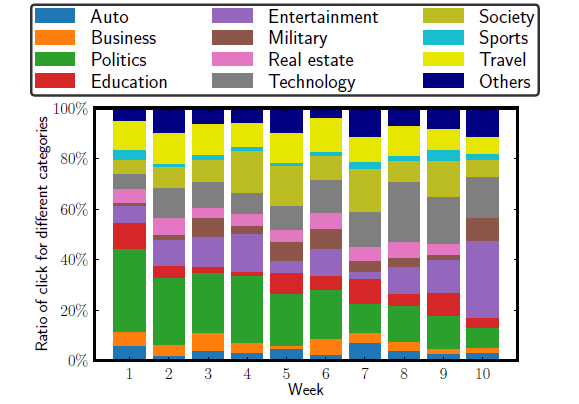
\includegraphics[scale = 0.6]{PPT/figure 1.png}
             \caption{Distribution of clicked categories of an active user
 in ten weeks. User interest is evolving over time.}
         \end{figure}
 \end{frame}

\begin{frame}{How is this method different?}
   \begin{itemize}
       \item In this paper, they propose a Deep Q-Learning based recommendation framework, which can model future reward explicitly.
       \item More information than click / no click label.
       \item In contrast to MAB-based methods, MDP-based methods can not only capture the reward of current iteration, but also the potential reward in the future iterations.
      \item Partial MDP can not scale to large dataset.
      \item They propose a MDP framework with continuous state and action representation.
\end{itemize}
\end{frame}






% \begin{frame}{Deep Reinforcement Recommendation System}
% 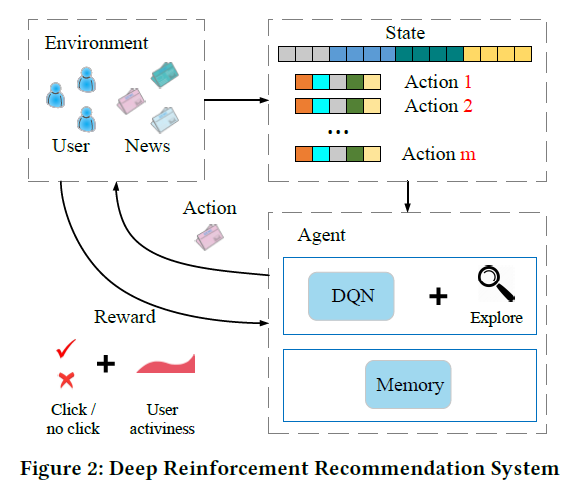
\includegraphics[height=6.8cm]{figure 2.png}
% \centering
% \end{frame}

% \begin{frame}{Deep Reinforcement Recommendation System}
% \begin{itemize}

%  \item In order to better model the dynamic nature of news characteristics and user preference, Deep Q-Learning (DQN) framework has been used.
%       \item This framework uses a DQN structure and can easily scale up.
%       \item The framework consider user return as another form of user feedback information, by maintaining an activeness score for each user.
%       \item The framework consider multiple historical return interval information to better measure the user feedback.
%       \item The model can estimate user activeness at any time (not just when user returns). This property enables the experience replay update used in DQN.
%       \item By applying a Dueling Bandit Gradient Descent (DBGD) method for exploration, by choosing random item candidates in the neighborhood of the current recommender, the strategy avoid recommending totally unrelated items and hence maintain better recommendation accuracy.
%       \end{itemize}
% \end{frame}

%merge the next three and form two slides



 
%  \begin{frame}{Notations}
% 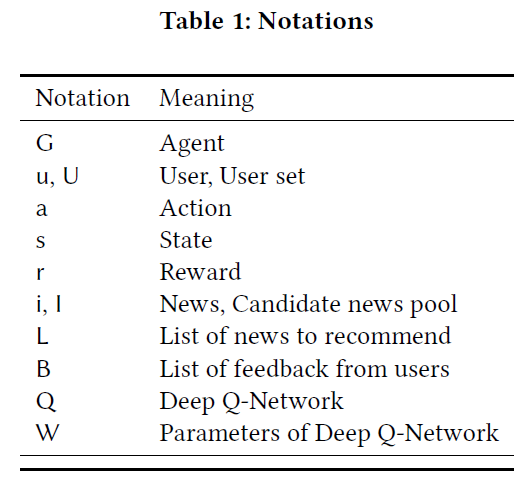
\includegraphics[height=6.8cm]{figure 3.png}
% \centering
% \end{frame}




\begin{frame}{Preliminary on DQN \cite{DBLP:journals/corr/MnihKSGAWR13}}
\begin{enumerate}
    \item In contrast to TD-Gammon and similar approaches, a technique known as experience replay is used, where the agent’s experiences are stored at each time-step, $e_t = (s_t, a_t, r_t, s_{t+1})$ in a data-set $\mathcal{D} = e_1, \dots, e_N$ , pooled over many episodes into a replay memory.
    \item Q-learning updates, or minibatch updates are applied to samples of experience, $e \in \mathcal{D}$, drawn at random from the pool of stored samples.
    \begin{center}
        $L(\theta) = \mathbb{E} \limits_{(s,a)}\Big[(y_j − Q(s , a ; \theta))^2\Big]$\\
        $\theta &= \theta - \eta \nabla L(\theta)$
    \end{center}
    \item After performing experience replay, the agent selects and executes an action according to an $\epsilon$-greedy policy.
    \begin{center}
        With probability $\epsilon$ select a random action $a_t$\\
        otherwise select $a_t = \max_a Q(s_t, a; \theta)$
    \end{center}
    \item Learning from the randomized samples of experience replay memory reduces the correlations among samples and therefore reduces the variance of the updates.
\end{enumerate}
\end{frame}

\begin{frame}{DQN: Algo}
\begin{algorithm}[H]
\caption{Deep Q-learning with Experience Replay}
	\begin{algorithmic}[1]
	    \State Initialize replay memory $\mathcal{D}$ to capacity $N$;
	    \State Initialize action-value function $Q$ with random weights;
		\For {$episode=1,2,\ldots, M$}
		    \State Initialise sequence $s_1 = \{x_1\}$, preprocess sequence $\phi_1 = \phi(s_1)$
		    \For {$t=1,2,\ldots, T$} 
		    \State With probability $\epsilon$ select a random action $a_t$
		    \State otherwise select $a_t = \max_a Q(s_t, a; θ)$ 
		    \State Execute action $a_t$ in emulator and observe reward $r_t$ and $x_{t+1}$
		    \State Set $s_{t+1} = s_t, a_t, x_{t+1}$ and preprocess $\phi_{t+1} = \phi(s_{t+1})$
		    \State Store transition $(\phi_t, a_t, r_t, \phi_{t+1})$ in $\mathcal{D}$
		    \State Sample random minibatch of transitions $(\phi_j , a_j , r_j , \phi_{j+1}) \in \mathcal{D}$
		    \State Set $y_j = r_j$ \quad for terminal $\phi_{j+1}$
		    \State Set $y_j = r_j + \max_{a'} Q(\phi_{j+1}, a'; \theta)$ \quad for non-terminal $\phi_{j+1}$
		    \State Perform a gradient descent step on $(y_j − Q(\phi_j , a_j ; \theta))^2$
		    \EndFor
		\EndFor
	\end{algorithmic} 
\end{algorithm}
\end{frame}
\begin{frame}{User Activeness}
    \begin{enumerate}
        \item New criteria used as a component of Reward along with traditional click information
        \item Activeness of user is modeled using Survival models (cite here)
        \begin{equation}
            S(t) = e^{- \int_0^t \lambda(x)dx}
        \end{equation}
        \item $\lambda(t) = \lambda_0$ is set as the constant probability of click happening after time t
        \item Every time a click happens user activeness is incremented as $S(t) = S(t) + S_a$
        \item Total Reward : $r_{total} = r_{click} + r_{active}$
        \begin{figure}
            \centering
            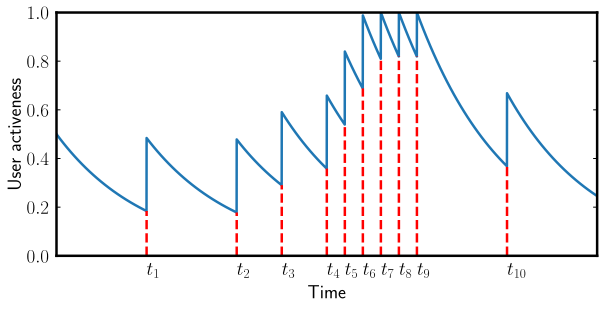
\includegraphics[scale=0.3]{DeepinScreenshot_select-area_20200514225125.png}
            %\caption{}
            \label{fig:user_activeness}
        \end{figure}
    \end{enumerate}
\end{frame}



\begin{frame}{Exploration}
\begin{columns}
\begin{column}{0.7\textwidth}
   \begin{enumerate}
       \item Dueling Bandit Gradient Descent (DBGD) is used to do exploration
       \item Two Q networks, $\Tilde{Q}$ is a perturbation of $Q$
       \item $\Tilde{W} = W + \alpha \cdot rand(-1,1) \cdot W$
       \item Recommended lists $L$ and $\Tilde{L}$ are merged into $\hat{L}$ via probabilistic interleaving
       \item If item recommended by $\Tilde{Q}$ receives better feedback update $Q$ towards $\Tilde{Q}$
       \item $W^* = W + \eta\Tilde{W}$
       \item Otherwise $Q$ is unchanged
   \end{enumerate}
\end{column}
\begin{column}{0.3\textwidth} 
    \begin{center}
     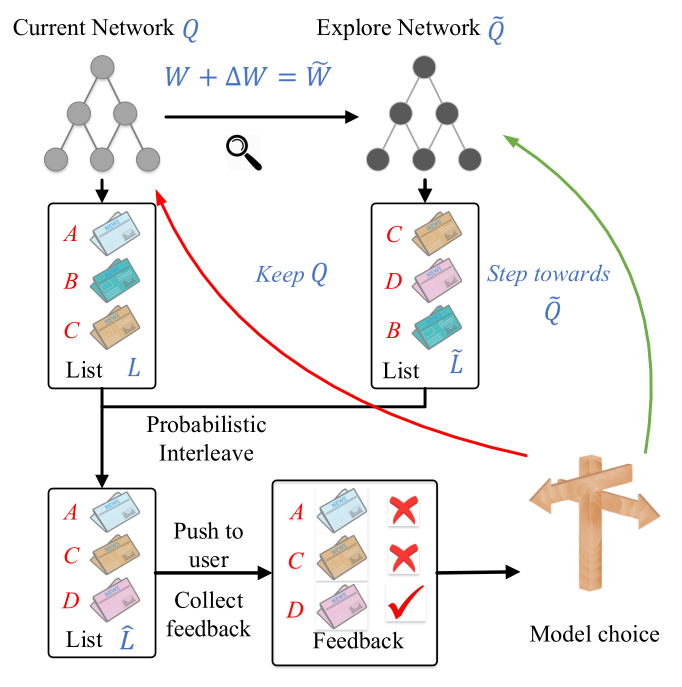
\includegraphics[scale=0.2]{DeepinScreenshot_select-area_20200514225903.png}
     \end{center}
\end{column}
\end{columns}
\end{frame}


\begin{frame}{Evaluation Measures}
    \begin{enumerate}
        \item Click Through Rate (CTR)
        \begin{equation}
            CTR = \frac{number\, of\, clicked\, items}{number\, of\, total\, items}
        \end{equation}
        \item Precision at k
        \begin{equation}
            Precision@k = \frac{number\, of\, clicks\, in\, top\, k\, recommended\, items}{k}
        \end{equation}

    \item Normalized Discounted Cumulative Gain (nDCG)
    \begin{equation}
        DCG(f) = \sum\limits_{r=1}^n y_r^f \frac{1}{log(1+r)}
    \end{equation}
    \end{enumerate}
\end{frame}
\begin{frame}{Experiments}

\end{frame}


\bibliographystyle{unsrt}
\bibliography{references}
\end{document}